\documentclass[paper=a4paper,jafontsize=9pt,head_space=15mm,gutter=20mm,
twocolumn,number_of_lines=49, line_length=26zw]{myuarticle}

\begin{document}

\title{{\LARGE\bfseries\gtfamily 他者にとっての快・不快を身体的動作によって提示するロボットインタフェースの実装}}
\author{\\\ 22120165 中村龍造 \\ (指導教員 : 佐藤宏樹)\\ \\}
\date{}
\maketitle

\section{まえがき}
本稿では,同じ生活空間に存在する多様な「他者」を基準とした環境評価と,それをロボットの動作によって表現するシステムについて報告する.

IoTやセンシング技術の進展により,人間の生活空間はより快適で効率的なものとなっている.しかしながら現状のIoTシステムは,多くの場合システムの中心であるはずの人間を障害物のようにみなしている\cite{Petrov-2018-WhenIoTKeepsPeople}.
また人間どうしであっても,身体的差異や文化,価値観などの違いによって,同じ環境であってもそれを快適と感じるかどうかには個人差がある.

本システムでは,取得した環境データに対して,人間,動植物,非生物などといった複数の主体からの評価基準を設定し,評価結果をロボットの身体的動作を通して表現する.また,岡田ら\cite{岡田-2017-弱いロボ}の提唱する『弱いロボット』の表現方法を用いて,人間をタスク遂行の一部に効果的に組み込むことで,機能・コスト等の要求を低減しつつ,人と関わり合うロボットとしてのあり方を模索する.

本システムを通じて,ユーザーが「他者」にとっての快適さを知り,「他者」への理解,関心を深めることで,多様な存在との対話の機会創出を目指す.

\section{関連研究と課題}
環境センシング分野では,IoTやセンサー技術の発展により,室内環境の継続的なモニタリングが可能となっている\cite{Saini-2020-IndoorAirQualityMonitoring}.また,屋内環境品質に関して,Coulbyら\cite{Coulby-2020-ScopingReviewTechnologicalApproaches}は客観的データだけでなく,個々人の主観による評価も必要であると指摘している.

Human Robot
Interaction
の分野では,Breazeal\cite{C.Breazeal-2004-SocialInteractionsHRIRobot}が現実世界で活動するロボットのあり方について,単一でタスクを遂行するのではなく,人間と協働してタスクを遂行するパートナーとしてのあり方を提示している.

環境データの表現手法については,可視化にはモバイルアプリやウェブ上での情報提示がほとんどであり\cite{Saini-2020-IndoorAirQualityMonitoring},ロボットの動きを用いたものは少ない.

こうした情報提示の形に加え,Dezeen\cite{-2015-VirtualRealityPresentsForest}による,ユクスキュルの「環世界」の概念とVRを組み合わせて,「他者」が知覚する世界を表現したものもある.生物の身体的な「環世界」のみならず,ソン\cite{--ソンヨン}の作品では,非生物を「他者」として,「使用されていない服が自動で売られる」という処理を「服の死」という振る舞いとして表現している.渡邊ら\cite{渡邉-2019-情報環世}はこのような情報技術や言語,文化などの差異を「情報環世界」と呼んでいる.

以上から本研究では,人間,動植物,非生物など,様々な「他者」を基準に,それらから見た環境の快・不快を,ロボットの身体的動作で表現するシステムを開発する.

\section{システム要件}
本システムの開発にあたって,次の3点を要件とする.
\begin{itemize}
  \item ロボット:自身が代弁する「他者」の特徴が動きに現れている
  \item 評価システム:「他者」基準の評価が適切に行われる
  \item 全体:ユーザー自身とそれ以外との環境の受け取り方の違いを体験することができる
\end{itemize}

\subsection{全体のフロー}
システム全体は,ユーザー,環境,センサー,ロボット,本システムの5つの間で動作する.システム全体のフローを図\ref{fig:system-flow}に示す.

\fboxsep=0pt            %画像と枠線をくっつける.
\fboxrule=1pt            %枠線の太さを1ptにする.
\begin{figure}[h]
  \centering
  \fbox{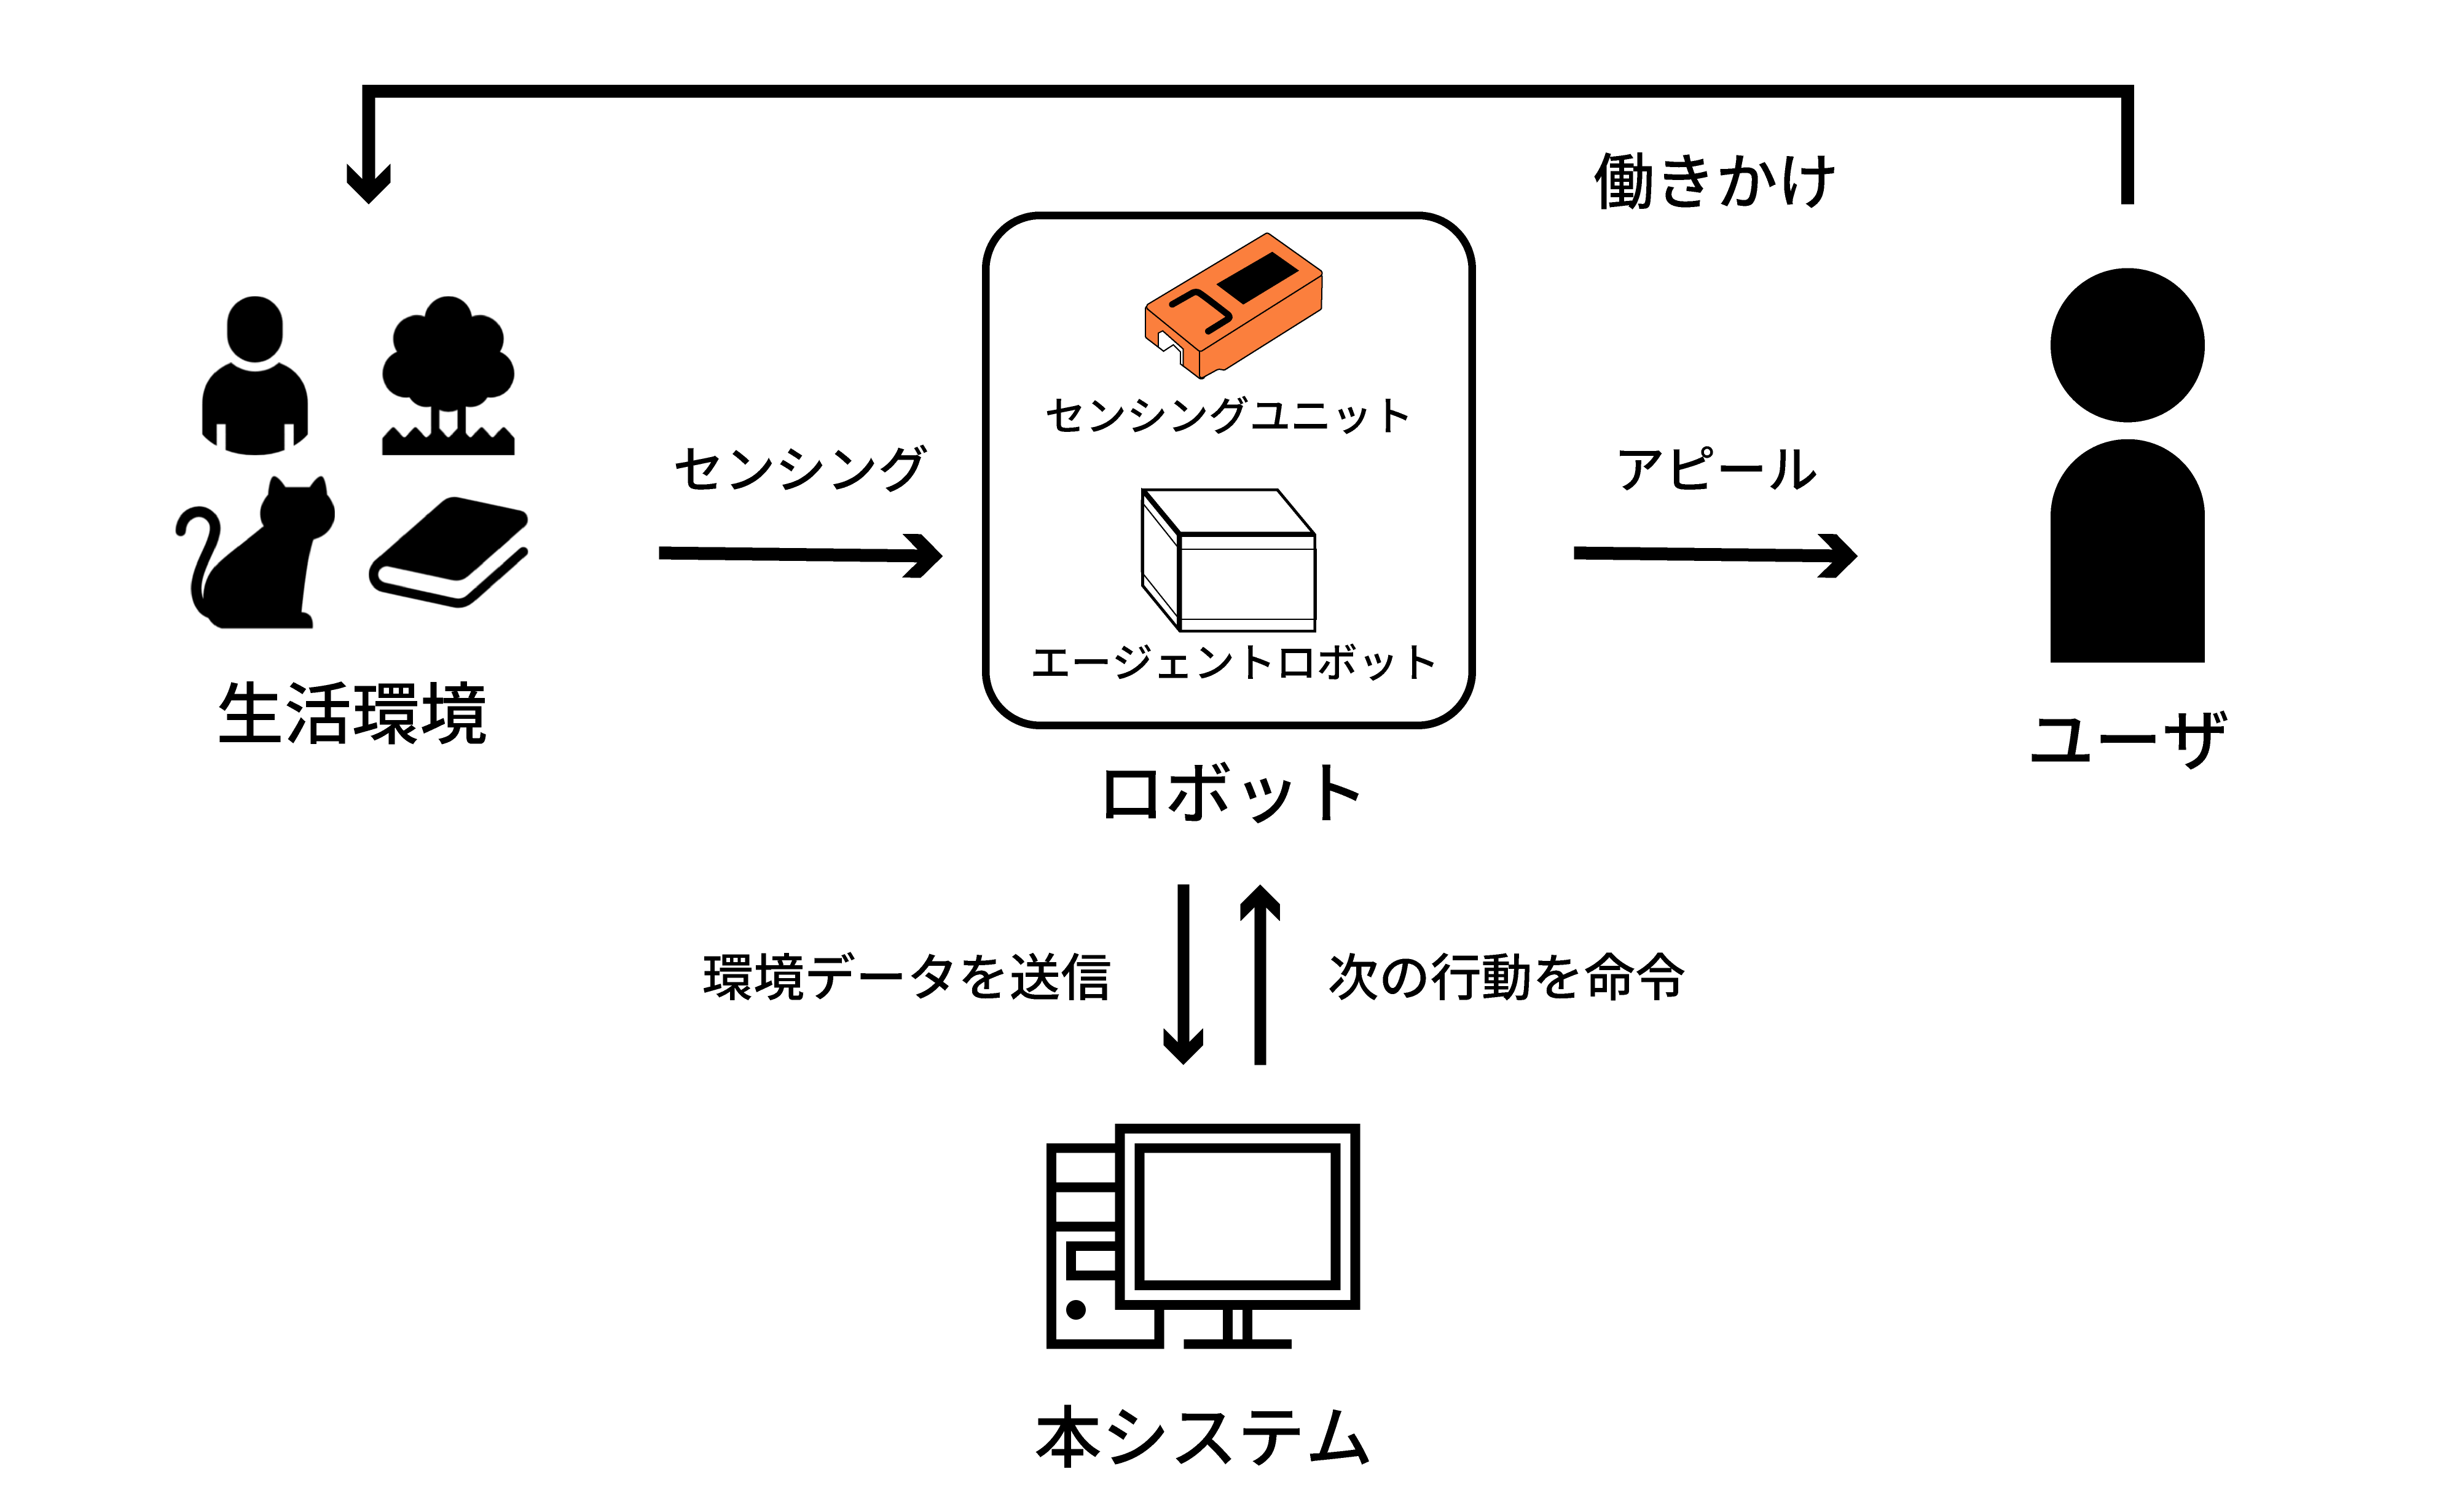
\includegraphics[keepaspectratio, clip,
  width=0.8\columnwidth]{resources/system_flow.png}}
  \caption{システム全体のフロー図}
  \label{fig:system-flow}
\end{figure}

はじめに本システムが,センサーを通じて生活空間の環境データを取得する.「他者」を基準とした評価,評価に応じて快・不快をアピールするなどの行動命令を現実空間のロボットに送信する.ロボットは行動命令に従って人間にアピールする.それを見た人間が環境や「他者」に対して働きかけることで,他者にとってより快適な環境を得るシステムとなっている.

\section{本システムの実装}
本システムは,センシングシステム,評価システム,アクション生成システム,ロボット制御システムから構成される.本システムの構造を図\ref{fig:system-structure}に示す.

\fboxsep=0pt            %画像と枠線をくっつける.
\fboxrule=1pt            %枠線の太さを1ptにする.
\begin{figure}[h]
  \centering
  \fbox{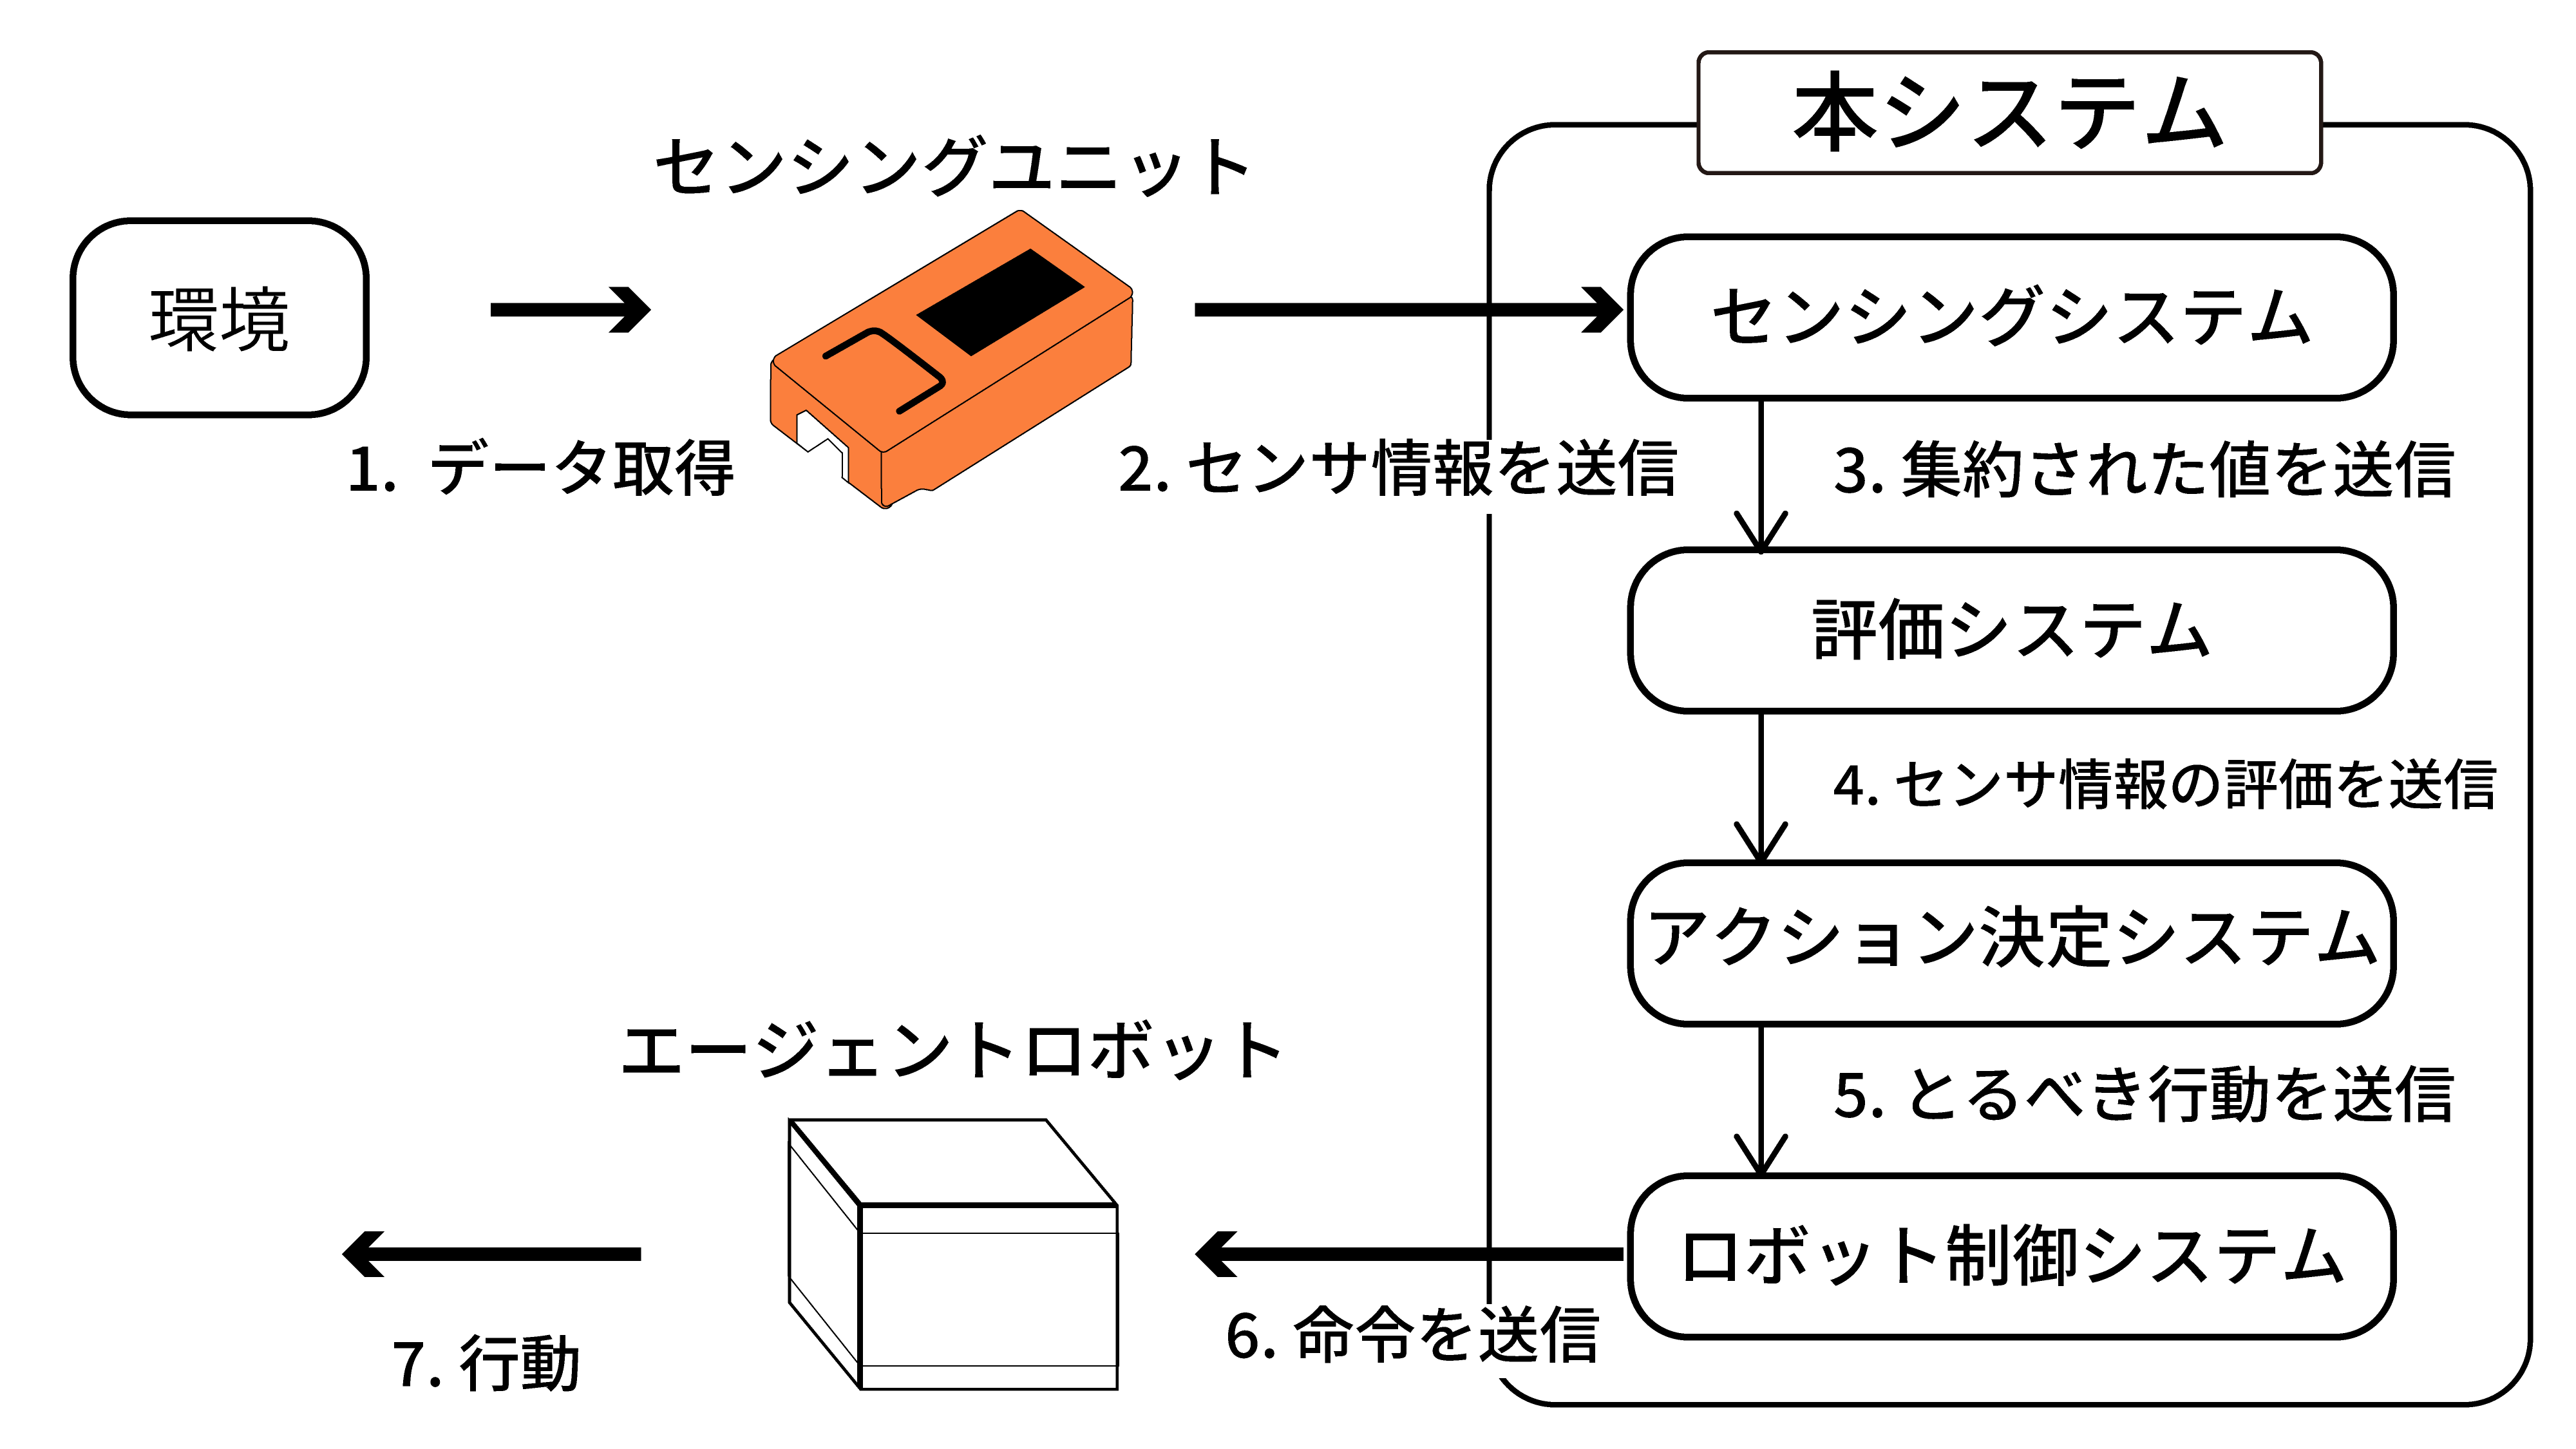
\includegraphics[keepaspectratio, clip,
  width=0.8\columnwidth]{resources/system_structure.png}}
  \caption{本システムの構造図}
  \label{fig:system-structure}
\end{figure}

センシングシステムは,センサ側とクライアント側の2つの部分から構成される.センサ側では環境データの取得と,シリアル通信での送信を行う.クライアント側ではデータの受信とデシリアライズを担当する.

評価システムでは,センサが取得した環境データのうち,自身が評価するデータを取得し,評価結果を返す.

評価データは,環境評価のスコアを持っている.スコア決定では,はじめに各主体ごとの気温や湿度といった環境データの適正値を設定する.環境データが適正値の範囲内であれば,スコアは0となる.適正値の範囲外だった場合,適正値より低ければ負のスコアを,高ければ正のスコアを返す.

アクション生成システムでは,主体と対象データに応じて,スコアごとに対応するアクションを生成する.対象データの形式には,気温のようにある適温を基準に閾値が正負の両側に広がるパターンもあれば,二酸化炭素濃度のような一方向に閾値が広がるパターンもある.パターンに応じて,生成するアクションの分岐を設定する.

アクションの生成にあたり,本システムでは1つのアクションを,「Action」と「Motion」という2種類のデータで処理している.Motionはロボットの詳細な動作命令および動作完了に必要なインターバルの情報を持つ.Actionは1つのアクションに必要な一連のMotionをキューとして持ち,ロボットは送られたActionの最も古いMotionから逐次実行する.

各テーマのアクションを実装するにあたり,アクションを集めて再利用可能にするため,「ActionLibrary」を作成した.本システムでは,toioで可能なアクションを個別に提供する「基本アクション」と,基本アクションを組み合わせて各主体・評価値に応じた「複合アクション」を実装している.

またサンプルとして実装したアクションでは,岡田ら\cite{岡田-2017-弱いロボ}の提唱する『弱いロボット』の概念を取り入れ,よたよたとした動きで「弱さ」を演出することで,ユーザーをシステムフローに効果的に取り入れることを狙った.

センシングデバイスとしてM5StickCを、ロボットとしてtoioを選定した。M5StickCは、スタンドアロンでの動作が可能で、HATによる高い拡張性を持ち、プログラミングが容易である。一方、toioは屋内空間に複数配置でき、多様な「他者」を同時に表現できる特徴がある。また、インタラクションに必要な基本的な動作が実装済みであり、toio-sdkを用いてシミュレーションでの開発が可能である。

\section{本システムの制約}

本システムの適用可能な範囲について、以下の制約が存在する。

物理的な制約として、温度、湿度、CO2濃度などのセンサーの測定可能範囲があり、toioは専用マットが必要という動作範囲の制限がある。また、システムは室内環境に限定されており、屋外での利用は想定していない。さらに、電源供給が必要でバッテリー駆動時間にも制限がある。

対象とする「他者」に関する制約については、環境データで評価可能で、評価基準が明確に設定でき、客観的なデータが入手可能な主体に限定される。

システムの表現力については、toioで表現可能な動作の範囲や、toioの台数制限による一度に表現できる「他者」の数、動作パターンの種類に制限がある。

利用環境については、Bluetooth通信が可能な範囲内であることが必要で、toioの動作のために一定の広さのある平面が必要である。また、複数の「他者」を同時に表現する場合には空間的な制約がある。

ユーザー側の制約としては、システムの意図を理解でき、ロボットの動作を観察できる位置にいる必要があり、環境調整が可能な権限を持つユーザーであることが求められる。

データ処理に関しては、データ取得から表現までの遅延というリアルタイム性や、評価基準の更新頻度、同時に処理可能なセンサーデータの数に制約がある。

\section{今後の展望}
今後の展望として、以下のような方向性が考えられる。アクションデザインの観点からは、ロボット同士の共同イベントの実装、より自然な動作パターンの設計を検討する必要がある。センシング面においては、快・不快をより適切に表現可能なデータの選定を行うとともに、取得データのノイズ除去による明確な変化の知覚を実現することが求められる。ハードウェアに関しては、異なるロボットプラットフォームへのweak-toioシステムの実装、およびHERMITSに見られるようなハードウェアの改造による機能拡張が考えられる。さらに、Mixed
Reality技術との統合により、キャラクターや動作のデザインの自由度を向上させるなど、異分野との融合による新たな展開も期待される

\section{あとがき}
本研究では,環境データを「他者」の視点から評価し,ロボットの身体的動作を通じて表現するシステムを開発した.M5StickCとtoioを用いたプロトタイプシステムの実装により,「他者」にとっての快・不快を直感的に理解できるインタフェースを実現した.特に,『弱いロボット』の概念を取り入れることで,ユーザーを自然にシステムフローに組み込むことができた.

今後は,より多様な「他者」の表現や,ロボット同士の協調動作の実装など,システムの拡張を進めていく.

%  ----- 参考文献 -----
% 参考文献リストの「参考文献」のスタイル
\renewcommand{\refname}{ 参考文献}
\bibliography{ref}
\bibliographystyle{junsrt}
\end{document}
